%%%%%%%%%%%%%%%%%%%%%%%%%%%%%%%%%%%%%%%%%%%%%%%%%%%%%%%%%%%%%%%%%%%%%%
% How to use writeLaTeX: 
%
% You edit the source code here on the left, and the preview on the
% right shows you the result within a few seconds.
%
% Bookmark this page and share the URL with your co-authors. They can
% edit at the same time!
%
% You can upload figures, bibliographies, custom classes and
% styles using the files menu.
%
%%%%%%%%%%%%%%%%%%%%%%%%%%%%%%%%%%%%%%%%%%%%%%%%%%%%%%%%%%%%%%%%%%%%%%

\documentclass[12pt]{article}

\usepackage{sbc-template}
\usepackage{graphicx,url}
\usepackage{natbib}


%\usepackage[brazil]{babel}   
\usepackage[utf8]{inputenc}  

     
\sloppy

\title{Gamificação do aprendizado de línguas utilizando SRS\\e plataformas de streaming}

\author{J. Emanuel Cascone R. S.\inst{1}, Guilherme A. Avelino\inst{1} }


\address{Departamento de computação - Universidade Federal do Piauí (UFPI)
  \email{\{emanuelcascone,gaa\}@ufpi.com.br}
}

\begin{document} 

\maketitle

\begin{abstract}
  The ability to learn a new language is directly related to the user's disposition and comfort for better interaction with learning platforms. This allows for the gamification of language learning, making it less exhausting. Typically, learning a new language starts with writing and reading, followed by listening and speaking. This project aims to facilitate language learning by using a movie streaming platform with subtitles, enabling the user to watch movies with the original audio and subtitles. The project is based on the premise that to understand a text, you don't necessarily need to know the whole formation, but rather just the keywords or most repeated words, allowing you to apply skimming and scanning techniques. To solidify these words in the user's memory, gamified forms of Spaced Repetition System (SRS) can be applied to induce the user to better adapt to each scenario in the future based on their current repertoire. Following this approach, the user will have a better experience watching movies or videos to acquire knowledge of a new language. \\
\textbf{Key words:} language learning, gamification, streaming platforms, subtitles, SRS 
\end{abstract}
     
\begin{resumo} 
 Aprender uma nova língua está diretamente atrelado à disposição e conforto do usuário para que haja uma melhor interação com plataformas de aprendizado. Dessa forma é possível gamificar o aprendizado de novas línguas e torná-las menos exaustivas enquanto estudo. Cotidianamente, para adesão de uma nova língua, segue-se um padrão natural em que inicia-se pela escrita e leitura, após isso se transpõe para a audição e fala (considerando cenários em que o usuário não se encontra em países que utilizam a língua desejada). Visto isso, o seguinte projeto tenta viabilizar o aprendizado de novas línguas utilizando como base plataforma de streamings de filmes e suas legendas que, por meio destas, irá capacitar o usuário a assistir filmes com áudio e legendas em sua língua original.
O projeto baseia-se na premissa de que para compreender um texto não necessariamente precisa-se ter conhecimento sobre toda a sua formação, mas basta ter conhecimento de palavras chaves ou as mais repetidas para assim poder aplicar técnicas como skimming e scanning. De modo a cristalizar tais palavras na memória do usuário pode-se aplicar formas gamificadas de
Spaced Repetition System (SRS), para induzir que em situações futuras o usuário
consiga se adequar melhor a cada cenário de acordo com o seu repertório atual. Seguindo este viés é possível aferir que o usuário teria uma melhor experiência ao assistir filmes ou até
mesmo vídeos com o propósito de adquirir conhecimento de uma nova língua.
\\
\textbf{Palavras chaves:} aprendizado de línguas, gamificação, plataformas de streaming, legendas, SRS
\end{resumo}


\section{Introdução}
Aprender uma nova língua é uma tarefa importante e pode trazer muitos benefícios para o indivíduo, no entanto, nem sempre é uma tarefa fácil e desafiadora. Muitas vezes, a falta de disposição e conforto do usuário pode dificultar o aprendizado. Para superar esse obstáculo, o presente projeto visa gamificar o aprendizado de novas línguas, tornando-o menos exaustivo e mais prazeroso.\\
O projeto consiste na criação de uma extensão para navegadores que irá interagir com sites de streamings quando os usuários estiverem assistindo filmes com legendas. A extensão irá identificar as palavras mais comuns na legenda e aplicar técnicas de Spaced Repetition System (SRS), com o objetivo de ajudar o usuário a aprender a nova língua de forma gamificada.\\
Estudos demonstram que alunos tendem a ter o dobro da velocidade de aquisição de uma nova língua utilizando um mecanismo de aprendizado semelhante chamado de smart subtitle \cite{Kovacs13}, desse modo é viável inferir que abordagens com plataformas de entreternimento também podem ser efetivas para o aprendizado, em especial, utilizando a legenda de plataformas. \\
A metodologia adotada para o desenvolvimento da extensão será baseada em pesquisas sobre o processo de aprendizado de novas línguas, bem como em técnicas de gamificação. A organização do projeto será feita em etapas, começando pela pesquisa e seguindo para o desenvolvimento da extensão, sua validação e testes.\\
O objetivo principal deste projeto é oferecer uma solução para tornar o aprendizado de novas línguas mais fácil e agradável para o usuário, permitindo-lhe aproveitar o tempo livre para adquirir conhecimento de uma nova língua de forma lúdica e eficaz. Ao final deste projeto, espera-se que o usuário tenha uma melhor compreensão da nova língua, o que poderá ser verificado por meio de avaliações e feedbacks dos usuários.

\subsection{Motivação}
A motivação para esse projeto surge da necessidade de encontrar alternativas para tornar o processo de aprendizado de uma nova língua mais interessante e eficiente. Atualmente, o método convencional de aprendizado de línguas pode ser cansativo e desmotivador para muitos estudantes. \\
Com a criação de uma extensão para navegadores que permita a interação com sites de streamings de filmes, o aprendizado da nova língua pode ser feito de maneira mais natural e lúdica, assim como ferramentas que traduzem páginas web para facilitar o aprendizado ou compreensão de outras línguas já presentes no mercado ou na área de pesquisa \cite{ElBatanony21}.\\
Ao assistir filmes com áudio e legendas na língua original, o usuário pode aprender de forma não-intrusiva, ao mesmo tempo em que aplica técnicas gamificadas de SRS para fixar as novas palavras na memória. A motivação para esse projeto é fornecer uma alternativa eficiente e atrativa para o aprendizado de novas línguas.

\subsection{Objetivo Geral}

O objetivo geral deste projeto é desenvolver uma extensão para navegadores que permita aos usuários aprender uma nova língua ou aumentar seu vocabulário de forma gamificada e interativa. A extensão será projetada para interagir com sites de streamings de filmes, aproveitando as legendas disponíveis nesses sites para auxiliar no processo de ensino. \\ 
O projeto baseia-se na premissa de que é possível aprender uma nova língua com maior eficiência e satisfação quando o processo é feito de forma gamificada e interativa. Além disso, tem base em uma metodologia semelhante - smart subtitles - que possui efetividade na ampliação do vocabulário \cite{Kovacs14}. \\ 
Desta forma, o objetivo é oferecer uma abordagem diferente e eficiente para utilizar legendas de modo em que as pessoas possam aprender novas línguas e aumentar seu vocabulário de forma descontraída e efetiva enquanto assistem a seus filmes favoritos.

\subsection{Objetivos Específicos}
Para atender ao objetivo geral serão realizados os seguintes objetivos específicos, a saber:
\begin{itemize}
\item Desenvolver uma extensão para navegadores que possa ser instalada por usuários interessados em aprender novas línguas.
\item Integrar a extensão com sites de streamings de filmes para que possa ser possível acessar as legendas dos filmes assistidos.
\item Criar uma base de dados de palavras-chave para cada língua aprendida e armazenar as informações do usuário, incluindo sua progressão no aprendizado.
\item Aplicar técnicas de Spaced Repetition System (SRS) gamificadas para ajudar o usuário a memorizar palavras-chave em sua nova língua.
\item Permitir que o usuário escolha a língua que deseja aprender, bem como o nível de dificuldade e a velocidade de aprendizado.
\item Proporcionar acesso a recursos de prática da fala, como dicionários de voz e traduções automáticas, para ajudar o usuário a desenvolver sua capacidade de fala.
\item Oferecer estatísticas sobre o progresso do usuário, incluindo as palavras mais difíceis e a taxa de acerto, para incentivar a persistência e o aprendizado contínuo.
\item Fornecer suporte a vários idiomas para a extensão, incluindo a interface e as traduções de filmes disponíveis.
\end{itemize}



\section{Desenvolvimento}
\subsection{Metodologia}
A metodologia a ser utilizada neste projeto consistirá na criação de uma extensão para navegadores que irá interagir com sites de streamings de filmes e extrair as legendas disponíveis nesses sites. A extensão utilizará técnicas de Spaced Repetition System (SRS) para gamificar o processo de aprendizado de novas línguas, baseado na premissa de que o conhecimento das palavras-chave ou as mais repetidas permite compreender um texto. 
\\
A extensão exibirá as palavras-chave durante a exibição do filme e utilizará técnicas de SRS para repetir as palavras de forma espaçada, com o objetivo de fixá-las na memória do usuário. Além disso, a extensão irá fornecer a tradução dessas palavras para a língua do usuário, para facilitar a compreensão.
\\
O desenvolvimento da extensão será feito com base nas seguintes etapas:
\begin{itemize}
\item Identificação dos sites de streamings que possuem legendas disponíveis para os filmes.
\item Desenvolvimento de uma ferramenta de extração de legendas.
\item Implementação da técnica de SRS para gamificar o processo de aprendizado de novas línguas.
\item Integração da extensão aos sites de streamings.
\item Testes e ajustes finais.
\end{itemize}
Ao final do projeto, espera-se ter uma extensão que possibilite aos usuários aprender novas línguas de forma mais eficiente e agradável, tornando o processo menos exaustivo e aumentando a disposição do usuário para o aprendizado.

\subsection{Atividades Chaves e Cronograma do Projeto}
\subsubsection{Atividades Chaves}

A lista das atividades propostas é dada abaixo; cada atividade é transportada para o cronograma que é detalhado na Tabela-\ref{tab:exTable1}.

\begin{itemize}
\item Pesquisa e estudo da documentação sobre extensões para navegadores.
\item Definição da arquitetura e escolha da tecnologia a ser utilizada.
\item Criação da interface gráfica da extensão.
\item Desenvolvimento da lógica de captura de legendas.
\item Desenvolvimento da lógica de ensino baseada nas legendas.
\item Integração da lógica de captura de legendas e ensino.
\item Teste final da extensão.
\item Revisão e correção de eventuais problemas identificados no teste final.
\item Elaboração da documentação técnica da extensão.
\item Entrega do projeto final.
\end{itemize}

\begin{table}[ht]
\centering
\caption{Cronograma para o desenvolvimento do projeto }
\label{tab:exTable1}
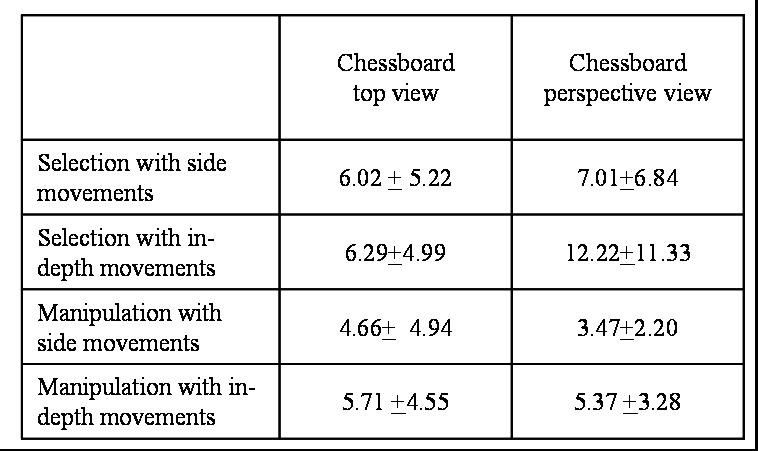
\includegraphics[width=.7\textwidth]{table.jpg}
\end{table}

\subsubsection{Cronograma do Projeto e atividades subjacentes}
\begin{itemize}

\item Dezembro de 2022:
\begin{itemize}
\item Definição do escopo do projeto
\item Início da pesquisa e estudo da documentação necessária sobre extensões para navegadores.
\end{itemize}

\item Janeiro de 2023:
\begin{itemize}
\item Início da definição da arquitetura e escolha da tecnologia a ser utilizada.
\item Início da criação da interface gráfica da extensão.
\item Realizar pesquisa bibliográfica e de referências de projetos semelhantes ou para embasamento teórico.
\end{itemize}

\item Fevereiro a Março de 2023:
\begin{itemize}
\item Desenvolvimento da lógica de captura e exibição de legendas dos sites de streaming.
\item Teste e aprimoramento da captura de legendas.
\end{itemize}

\item Abril a Maio de 2023:
\begin{itemize}
\item Desenvolvimento da lógica de ensino baseada nas legendas capturadas.
\item Teste e aprimoramento da lógica de ensino.
\end{itemize}


\item Junho a Agosto de 2023:
\begin{itemize}
\item Integração da lógica de captura de legendas e ensino.
\item Teste final da extensão.
\end{itemize}

\item Setembro a Novembro de 2023:
\begin{itemize}
\item Revisão e correção de eventuais problemas identificados no teste final.
\item Elaboração da documentação técnica da extensão.
\end{itemize}

\item Dezembro de 2023:
\begin{itemize}
\item Entrega do projeto final.
\end{itemize}

\end{itemize}


\bibliographystyle{sbc}
\bibliography{sbc-template}


\end{document}
